While in \autoref{chp:arrival_times}, \acp{FD} have mainly been used to determine the arrival time of \acp{ICME} at \SI{1}{\AU} and Mars, other properties of \acp{FD} have been neglected in these studies. However, some empirical relations between different properties of a \ac{FD} at Earth as well as between the \ac{FD} and properties of the associated \ac{ICME} are known, as shown e.g. by \citet{Belov-2008-FD,Abunin-2012-FD}. For example, there is a clear correlation between the relative \ac{FD} amplitude or the maximum decrease rate (``steepness'') with the product of the maximum solar wind speed and maximum magnetic field. This parameter $v_\text{max} \cdot B_\text{max}$ can be used to describe the intensity of the disturbance in the solar wind. The correlation is shown in Figure 8 of \citet{Belov-2008-FD} and Figure 7 of \citet{Abunin-2012-FD}.
However, solar wind plasma and magnetic field measurements at Mars are only available from the \ac{MAVEN} spacecraft since 2014, and as explained in \autoref{sec:motivation}, it does not observe the upstream solar wind continuously. So, the determination of maximum values for $B$ and $v$, which would be necessary for the validation of this relation at Mars, may be complicated for many events.

Instead, in this study, we focus on the ``inner relation'' of the two FD parameters: the relative amplitude and the maximum decrease rate. These are also known to be correlated at Earth, as seen in Figure 7 of \citet{Belov-2008-FD} and Figure 5 of \citet{Abunin-2012-FD}. We use our catalog of \acp{FD} from \citet{Forstner-2019}, as well as the larger catalog by \citet{Papaioannou-2019-FD-Earth-Mars} to reproduce this relation at Mars. Consulting the analytical \ac{FD} models, \acs{PDB} and \acs{ForbMod}, which were introduced in \autoref{sec:forbush}, it becomes possible to interpret the difference between the two observed relations as a result of the expansion of the interplanetary structures.

\TODO{Summary of the publication}

\newpage

The following article is reproduced from \textcite{Forstner-2020} from Journal of Geophysical Research: Space Physics, \copyright American Geophysical Union, under the Creative Commons CC-BY license: \ccLogo\ccAttribution\\

\pubcite{Forstner-2020}
\hfill Own contribution: 80\%

\newpage
\newcounter{includepdfpageJGRTwenty}

\addtocounter{section}{1}
\setcounter{subsection}{1} 
\phantomsection
\addcontentsline{toc}{section}{\arabic{chapter}.\arabic{section} Comparing the Properties of ICME-Induced Forbush Decreases at Earth and Mars (Publication JGR--Space Physics 2020)}
%
\phantomsection
\addcontentsline{toc}{subsection}{\arabic{chapter}.\arabic{section}.\arabic{subsection} Introduction}
\label{sec:paper_forstner2020}
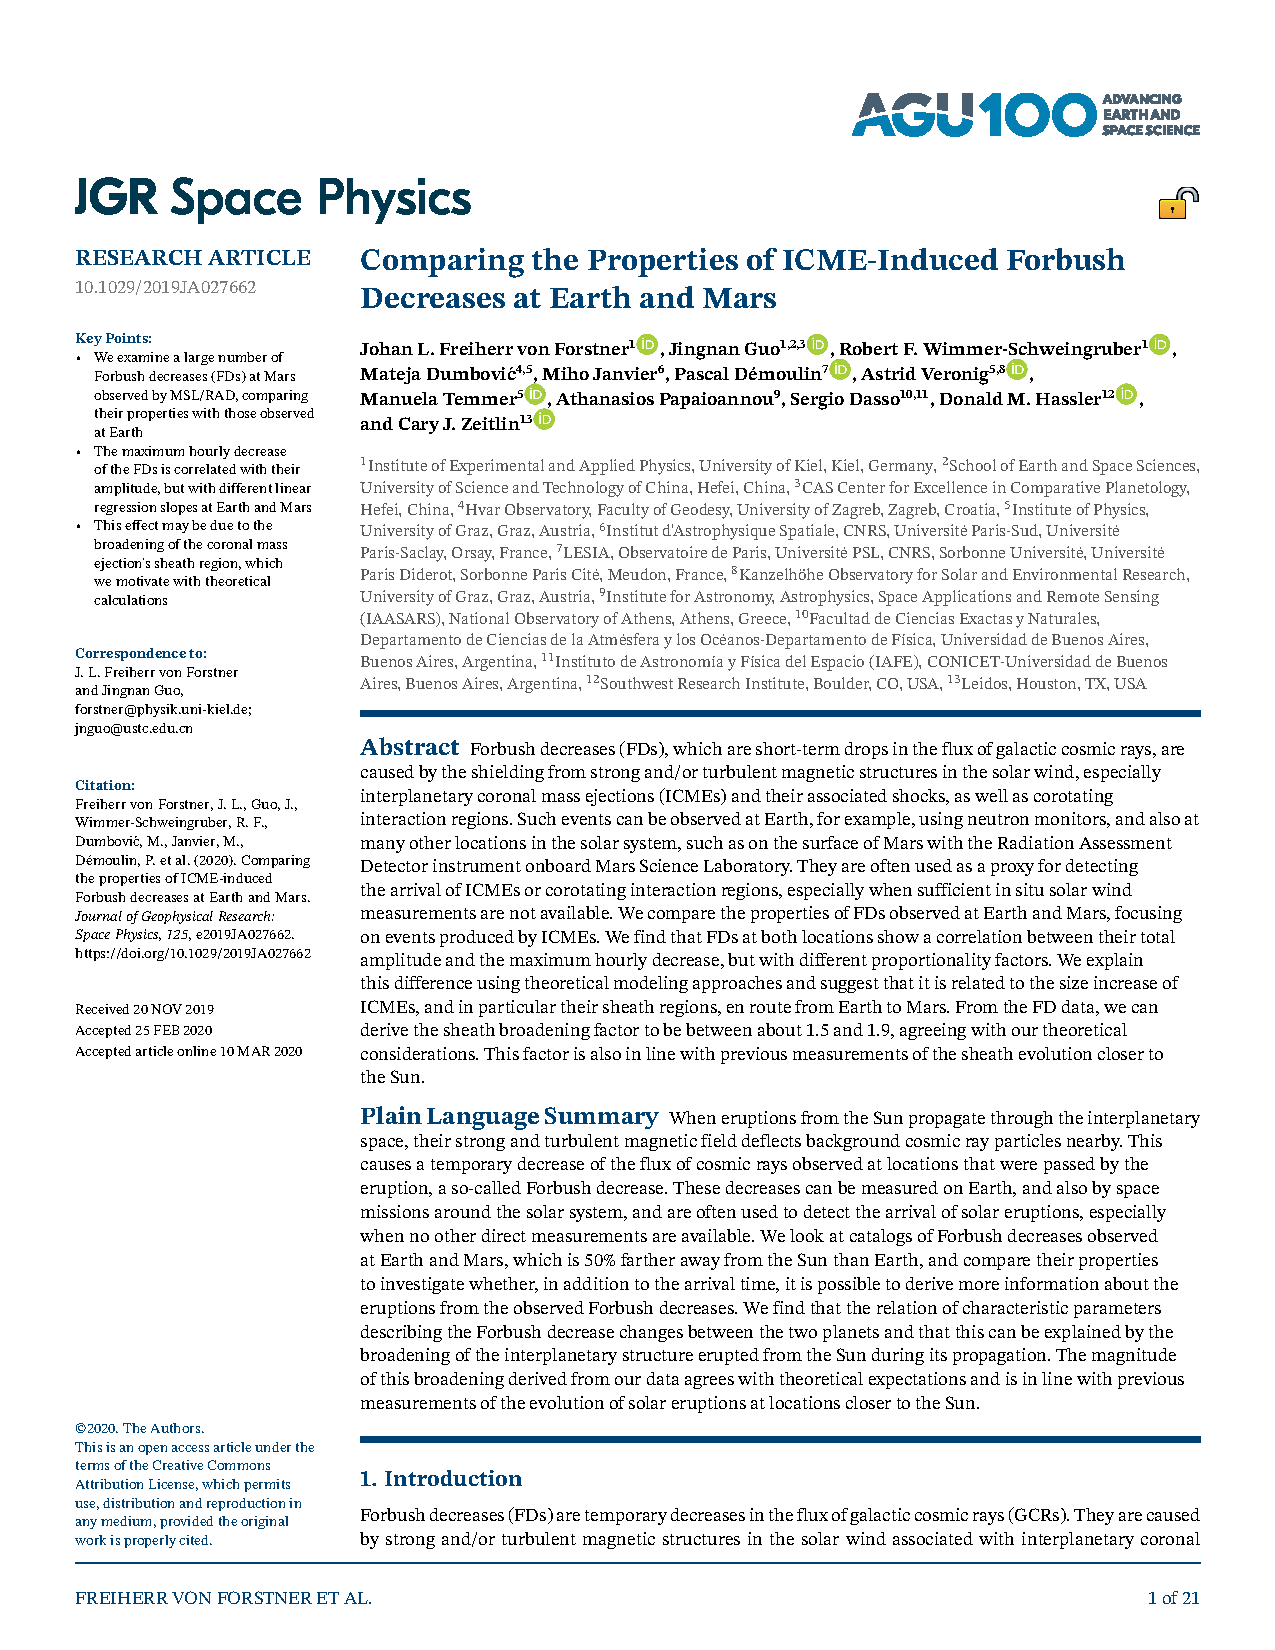
\includepdf[pages={1}, link, linkname=paper_forstner2020, scale=.95, pagecommand={\refstepcounter{includepdfpageJGRTwenty}\label{paper_forstner2020.\theincludepdfpageJGRTwenty}}]{publications/Forstner_et_al-2020-JGRSpace.pdf}
%
\addtocounter{subsection}{1} 
\phantomsection
\addcontentsline{toc}{subsection}{\arabic{chapter}.\arabic{section}.\arabic{subsection} Data Sources and Catalogs}
\includepdf[pages={2-5}, link, linkname=paper_forstner2020, scale=.95, pagecommand={\refstepcounter{includepdfpageJGRTwenty}\label{paper_forstner2020.\theincludepdfpageJGRTwenty}}]{publications/Forstner_et_al-2020-JGRSpace.pdf}
%
\addtocounter{subsection}{1} 
\phantomsection
\addcontentsline{toc}{subsection}{\arabic{chapter}.\arabic{section}.\arabic{subsection} Definitions and Methodology}
\includepdf[pages={6-7}, link, linkname=paper_forstner2020, scale=.95, pagecommand={\refstepcounter{includepdfpageJGRTwenty}\label{paper_forstner2020.\theincludepdfpageJGRTwenty}}]{publications/Forstner_et_al-2020-JGRSpace.pdf}
%
\addtocounter{subsection}{1} 
\phantomsection
\addcontentsline{toc}{subsection}{\arabic{chapter}.\arabic{section}.\arabic{subsection} Results and Discussions}
\includepdf[pages={8-16}, link, linkname=paper_forstner2020, scale=.95, pagecommand={\refstepcounter{includepdfpageJGRTwenty}\label{paper_forstner2020.\theincludepdfpageJGRTwenty}}]{publications/Forstner_et_al-2020-JGRSpace.pdf}
%
\addtocounter{subsection}{1} 
\phantomsection
\addcontentsline{toc}{subsection}{\arabic{chapter}.\arabic{section}.\arabic{subsection} Conclusions and Outlook}
%
\addtocounter{subsection}{1} 
\phantomsection
\addcontentsline{toc}{subsection}{\arabic{chapter}.\arabic{section}.\arabic{subsection} Appendix A: Location of $m_{\text{max}}$ Within the ICME Substructures}
\includepdf[pages={17-18}, link, linkname=paper_forstner2020, scale=.95, pagecommand={\refstepcounter{includepdfpageJGRTwenty}\label{paper_forstner2020.\theincludepdfpageJGRTwenty}}]{publications/Forstner_et_al-2020-JGRSpace.pdf}
%
\addtocounter{subsection}{1} 
\phantomsection
\addcontentsline{toc}{subsection}{\arabic{chapter}.\arabic{section}.\arabic{subsection} References}
\includepdf[pages={19-21}, link, linkname=paper_forstner2020, scale=.95, pagecommand={\refstepcounter{includepdfpageJGRTwenty}\label{paper_forstner2020.\theincludepdfpageJGRTwenty}}]{publications/Forstner_et_al-2020-JGRSpace.pdf}